%% Elsevier CAS double-column template (cas-dc), for Applied Soft Computing.
%% Compile: ../tools/tex/tectonic.exe -X compile cas_calmnet.tex --outdir .
%%
%% Every number is traceable to a JSON file in ../results/. Where two values
%% exist for the same model, both are reported and the reason is stated.
\documentclass[a4paper,fleqn]{cas-dc}
\usepackage[authoryear,longnamesfirst]{natbib}
\usepackage{amsmath,amssymb}
\usepackage{booktabs}
\usepackage{multirow}

\newtheorem{proposition}{Proposition}
\newdefinition{remark}{Remark}

\begin{document}
\let\WriteBookmarks\relax
\def\floatpagepagefraction{1}
\def\textpagefraction{.001}

\shorttitle{A parameter-efficient EEG decoder with in-network session adaptation}
\shortauthors{Author Name}

\title[mode = title]{A parameter-efficient EEG decoder with in-network session
adaptation, calibration and abstention for lower-limb exoskeleton control}

\author[1]{Author Name}
\cormark[1]
\ead{wshuvo360@gmail.com}
\credit{Conceptualization, Methodology, Software, Validation, Formal analysis,
Investigation, Data curation, Writing -- original draft, Writing -- review and
editing, Visualization}

\affiliation[1]{organization={Department},
            addressline={},
            city={},
            postcode={},
            country={}}

\cortext[1]{Corresponding author}

\begin{abstract}
\textbf{Background.} A decoder that drives a powered lower-limb exoskeleton is
fitted once and must keep working for weeks, during which electrode impedance,
montage and skin contact change the second-order statistics that every spatial
filter depends on. Correcting this shift inside the network, by re-estimating
the input covariance at inference and whitening by it without labels, is an
attractive design because it needs no target-domain calibration session.

\textbf{Problem.} We show that such a layer carries a failure mode its offline
counterpart cannot have. A running estimate tracks whatever is currently
streaming. Under a protocol that presents classes in long contiguous blocks, the
estimate converges to the currently active class and the layer whitens away the
signal it was inserted to protect.

\textbf{Solution.} We present a decoder combining a label-free adaptive
alignment layer, a multi-scale power stem that preserves log-power ratios, and a
selective head trained under a coverage constraint, and we derive an admissible
band for the adaptation rate from two timescales that are measurable from the
recording protocol before any model is fitted.

\textbf{Results.} On a 7-subject, 9-session exoskeleton cohort recorded across
weeks, the 24{,}181-parameter configuration reaches $0.901$ balanced accuracy
with expected calibration error $0.039$ and $0.876$ accuracy at $90\,\%$
coverage, at $53\,\%$ of the parameters of the strongest baseline evaluated in
the same pipeline ($0.913$). The alignment layer reduces session-to-session
covariance distance by $52.0 \pm 4.5\,\%$ and $83.9 \pm 3.9\,\%$ on two
independent cohorts, in 15 of 15 subjects ($p \le 10^{-4}$), against a no-op
control that shows no reduction. On the second cohort the architecture does not
transfer: the bare stem scores $0.737$ against $0.626$ for the full model.
Slowing adaptation past the class-block length recovers $+0.090$ to $+0.098$ on
all three arms that use alignment and exactly $0.000$ on both arms that do not.
Applying the same change to the first cohort costs $-0.060$, so the two optima
are opposite and no single rate serves both protocols.

\textbf{Significance.} The admissible rate band is bounded below by the
class-block timescale and above by the drift timescale. Where class blocks
outlast drift the band is empty and the layer should be omitted rather than
tuned. Because both bounds are properties of the experimental design, the
condition is a design-time check rather than a post-hoc diagnosis, and it
predicts where in-network adaptation will fail before a model is trained.
\end{abstract}

\begin{highlights}
\item A 24{,}181-parameter EEG decoder emitting class, calibrated confidence and
      an abstention decision.
\item Label-free in-network alignment reduces session drift by 52--84\% in 15 of
      15 subjects.
\item Test-time adaptation can track the streaming class and erase the signal it
      protects.
\item The adaptation rate is two-sided: two cohorts' optima are opposite,
      costing 0.06--0.09.
\item The admissible rate band is computable from the recording protocol before
      fitting.
\end{highlights}

\begin{keywords}
brain--computer interface \sep electroencephalography \sep test-time adaptation
\sep covariate shift \sep selective prediction \sep calibration \sep lower-limb
exoskeleton
\end{keywords}

\maketitle

%=============================================================================
\section{Introduction}

Spinal cord injury leaves roughly 250{,}000 to 500{,}000 people per year with
impaired or absent lower-limb function, and powered exoskeletons driven by
non-invasive brain signals are one route to restoring overground mobility
\citep{he_exo,lopezlarraz,do}. Decoding the wearer's intent to walk or to stop
from scalp EEG is the control problem at the centre of such systems
\citep{contrerasvidal,presacco}. It is not well described by per-epoch
classification accuracy alone, for three reasons that shape the design presented
here.

\paragraph{Longitudinal drift} The decoder is fitted once and must keep working
weeks later. In the primary cohort used here this is literal: the model is
fitted on sessions 1--3 and evaluated on sessions 4--9, recorded across weeks.
Electrode montage, impedance and skin contact all change between sessions, and
the resulting shift in second-order statistics is the dominant source of
non-stationarity in EEG decoding \citep{shenoy,krauledat,blankertz2008}. Session
drift degrades fixed spatial filters and is the reason most BCI systems require
a per-session calibration block \citep{vidaurre}.

\paragraph{Asymmetric cost} A false Walk command moves a person's legs. Balanced
accuracy scores that identically to a missed Walk and cannot distinguish one
sustained false activation from fifty scattered false windows. The quantity a
wearer experiences is spurious activations per minute of standing, which we
report alongside accuracy throughout.

\paragraph{No option to decline} A classifier trained only for accuracy must
emit a decision for every window. A device that acts on a confidence value needs
that value to be calibrated \citep{guo}, and needs a principled way to do
nothing when the evidence is weak \citep{chow,elyaniv}.

Existing responses to drift are mostly applied offline in preprocessing.
Euclidean Alignment whitens each recording by the inverse square root of its
mean covariance \citep{hewu}; Riemannian Procrustes analysis and parallel
transport generalise this to the manifold of symmetric positive-definite (SPD)
matrices \citep{rodrigues,yair,zanini}. All of these estimate the alignment
statistic over a complete recording, which means the target recording must exist
before the decoder can run on it. Test-time adaptation removes that requirement
in computer vision by updating normalisation statistics or parameters online
\citep{tent,schneider,nado}, and recent work shows that such methods degrade
when the test stream is temporally correlated rather than i.i.d.
\citep{note,sar,cotta}. EEG data acquired under a blocked experimental protocol
is temporally correlated by construction, which is the connection this paper
makes precise.

Our contributions are:

\begin{enumerate}
\item We introduce an adaptive alignment layer that estimates and applies a
      whitening transform without labels and continues to update at inference,
      and we verify that its output reaches the classifier rather than being
      undone by the following normalisation (Section~\ref{sec:align}).
\item We identify a failure mode specific to in-network alignment: the running
      estimate tracks the currently streaming class when class blocks exceed the
      estimator's memory, and the layer then removes the discriminative signal
      (Section~\ref{sec:rate}).
\item We derive an admissible band for the adaptation rate, bounded below by the
      class-block timescale and above by the drift timescale, and show the
      condition is two-sided by testing it in the direction where we predicted
      no effect (Proposition~\ref{prop:band}, Section~\ref{sec:twosided}).
\item We validate the mechanism separately from the task, reporting a
      $52.0\pm4.5\,\%$ and $83.9\pm3.9\,\%$ reduction in session-to-session
      covariance distance in 15 of 15 subjects against a no-op control
      (Section~\ref{sec:mechanism}).
\item We report an external validation that fails, with the ordering of arms
      inverting between cohorts, and trace the inversion to the rate condition
      rather than to sample size or implementation (Section~\ref{sec:external}).
\end{enumerate}

We make no accuracy claim over published decoders. In the pipeline where both
were evaluated, ATCNet \citep{atcnet} scores $0.913$ against $0.901$ for our
configuration, and we report that as a loss in Section~\ref{sec:compare}.

%=============================================================================
\section{Related work}

\subsection{Compact convolutional decoders for EEG}

ShallowFBCSPNet and Deep4Net established that a
$\mathrm{square} \rightarrow \mathrm{pool} \rightarrow \log$ pipeline over
learned spatial filters recovers the band-power features that filter-bank common
spatial patterns computes explicitly \citep{schirrmeister}. EEGNet reduced the
parameter count by an order of magnitude using depthwise-separable convolutions
\citep{lawhern}, and EEGNeX refined the same family \citep{eegnex}. These
architectures work well within a session and are the standard baselines in the
field \citep{roy_review,craik}. Their limitation for our setting is that the
learned spatial filters are fixed at training time, so a montage or impedance
change between sessions is not compensated at all. We respond by placing an
adaptive whitening stage before the spatial filters, so that what the filters
see is referred to a covariance estimated on the current recording
(Section~\ref{sec:align}).

\subsection{Attention-based decoders}

ATCNet combines convolutional feature extraction, sliding-window multi-head
attention and temporal convolution, and is the strongest baseline in our
comparison \citep{atcnet}. EEG Conformer pairs a ShallowFBCSP-style stem with a
transformer encoder \citep{conformer}, and EEG-TCNet applies temporal
convolutions to the same problem \citep{eegtcnet}. We note explicitly that the
stem-plus-transformer combination is already published: an independent
implementation of it in our pipeline reproduced EEG Conformer's score rather
than improving on it ($0.848$ against $0.843$), and we therefore claim no
novelty for that pairing. What these models share with the convolutional family
is a fixed front end, which is the property the present work targets.

\subsection{Alignment and transfer in BCI}

Riemannian methods treat the spatial covariance as a point on the SPD manifold
and classify with geodesic distances \citep{barachant,barachant2013,congedo}.
For transfer, Euclidean Alignment whitens each subject or session by
$\mathbf{M}^{-1/2}$ where $\mathbf{M}$ is its mean covariance \citep{hewu};
Riemannian Procrustes analysis adds rotation and scaling \citep{rodrigues}, and
parallel transport moves covariances between tangent spaces \citep{yair,zanini}.
These methods are effective and label-free, and reviews report them as the
strongest general-purpose transfer tools for EEG \citep{lotte2018,wu_transfer}.
Their limitation is operational rather than statistical: the alignment statistic
is computed over a whole recording, so the recording must be complete before
decoding starts, and within-recording drift is not tracked. We respond by moving
the estimator inside the network as a layer that updates online, and we then
show what that move costs (Section~\ref{sec:rate}).

\subsection{Test-time adaptation}

Updating normalisation statistics on the test distribution improves robustness
to corruption in vision \citep{schneider,nado}, and Tent extends this to
updating affine parameters by entropy minimisation \citep{tent}. Test-time
training adds a self-supervised objective at inference \citep{ttt}. A recurring
finding in this literature is that these methods assume the test stream is
i.i.d., and degrade when it is not: NOTE addresses temporally correlated streams
by maintaining a class-balanced reservoir \citep{note}, SAR stabilises
adaptation under distribution shift with small or imbalanced batches
\citep{sar}, and CoTTA and LAME address error accumulation in continual
adaptation \citep{cotta,lame}. Our contribution relative to this line is
quantitative rather than conceptual: we show that in a blocked EEG protocol the
relevant comparison is between the estimator's effective memory and the
duration of a single-class block, that this predicts the threshold location, and
that the resulting constraint is two-sided because the same estimator is also
what tracks the drift the layer exists to remove.

\subsection{Calibration and selective prediction}

Modern networks are overconfident, and expected calibration error
\citep{naeini,guo} degrades further under distribution shift \citep{ovadia},
which is exactly the regime a longitudinally deployed decoder operates in.
Selective classification allows a model to abstain \citep{chow,elyaniv}, and
SelectiveNet trains the classifier and the selection function jointly under a
coverage constraint \citep{selectivenet,geifman2017}. We use SelectiveNet as
published and claim no contribution to it; we include it because a decoder that
must not move a wearer's legs on weak evidence needs the reject option, and
because it is the only component in our ablation whose benefit transfers across
both cohorts.

\subsection{EEG correlates of gait and exoskeleton control}

Walking modulates cortical activity in a gait-phase-locked manner
\citep{gwin,seeber}, and treadmill walking can be decoded from scalp EEG
\citep{presacco,luu}. Robot-assisted gait modulates midline sensorimotor rhythms
\citep{wagner}. The intent signal our decoder targets is event-related
desynchronisation in the mu and beta bands, a power decrease over sensorimotor
cortex preceding and accompanying movement \citep{erd,pfurtscheller2006}. This
motivates a representation in which log-power ratios are preserved
(Section~\ref{sec:stem}), because ERD is defined as a relative power change.

%=============================================================================
\section{Problem formulation}

Let $\mathbf{X} \in \mathbb{R}^{C \times T}$ be a window of $C$ channels and $T$
samples with label $y \in \{\text{Stop}, \text{Walk}\}$. A recording session
$s$ supplies windows drawn from $p_s(\mathbf{X}, y)$. We assume the conditional
$p(y \mid \mathbf{X})$ is stable across sessions but the marginal
$p_s(\mathbf{X})$ is not, which is the covariate-shift assumption standard in
this literature \citep{sugiyama,shenoy}. Concretely we take the shift to act
primarily on the spatial covariance
$\mathbf{\Sigma}_s = \mathbb{E}_{p_s}[\mathbf{X}\mathbf{X}^\top] / T$.

The decoder is fitted on sessions $\mathcal{S}_{\mathrm{fit}}$ and evaluated on
disjoint later sessions $\mathcal{S}_{\mathrm{test}}$, with no labels available
from $\mathcal{S}_{\mathrm{test}}$ at any point. This is the constraint that
rules out per-session recalibration and motivates a label-free correction.

We quantify session drift by the affine-invariant Riemannian distance between
SPD matrices,
\begin{equation}
\delta(\mathbf{A},\mathbf{B}) =
\left\| \log\!\left( \mathbf{A}^{-1/2}\mathbf{B}\mathbf{A}^{-1/2} \right)
\right\|_F ,
\label{eq:riem}
\end{equation}
rather than the Frobenius distance, because covariances do not form a vector
space and the Frobenius distance is dominated by overall scale, which would
flatter any whitening operation \citep{congedo,barachant}.

Two timescales govern the analysis in Section~\ref{sec:rate}. Let
$\tau_{\mathrm{blk}}$ be the median duration, in windows, of a contiguous
single-class block in the recording protocol, and let $\tau_{\mathrm{drift}}$ be
the timescale over which $\mathbf{\Sigma}_s$ changes appreciably. Both are
properties of the experimental design and the recording hardware, not of the
model.

%=============================================================================
\section{Method}

The decoder maps a window to a class posterior and a selection score. Its four
components are shown in Fig.~\ref{fig:arch} with exact parameter counts.

\begin{figure*}[t]
\centering
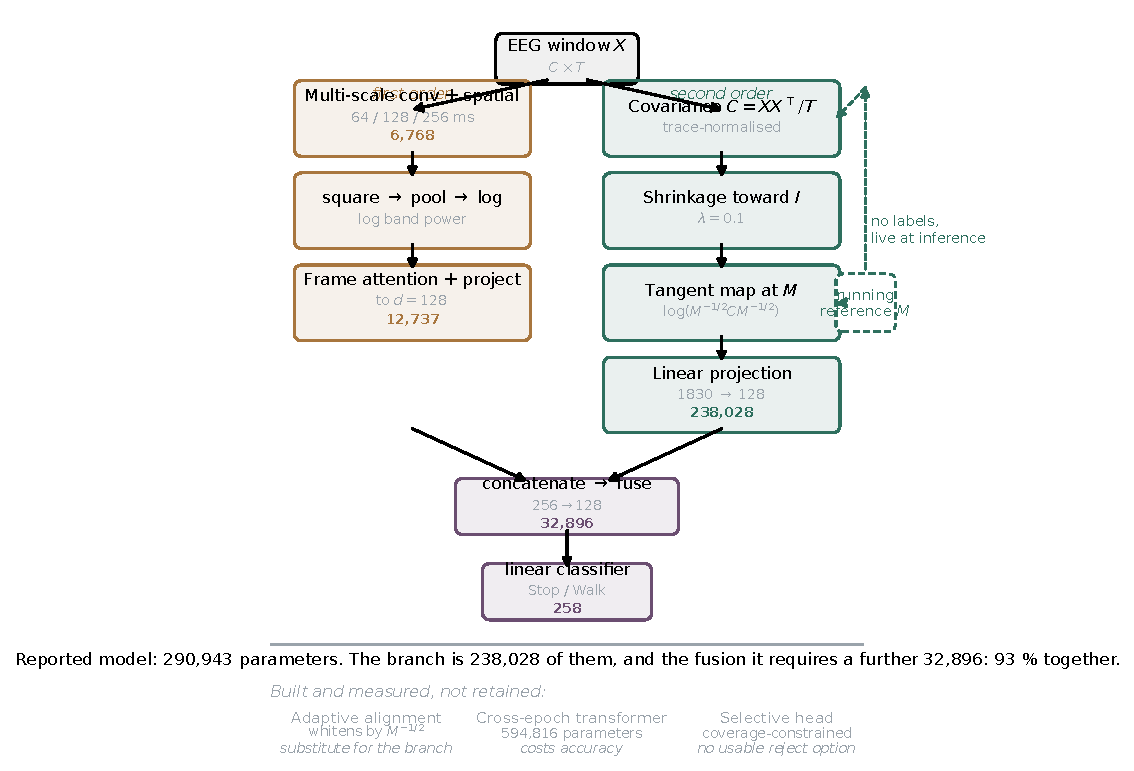
\includegraphics[width=\textwidth]{../results/fig_arch.pdf}
\caption{The decoder. The adaptive alignment layer maintains a running spatial
covariance and whitens by it; its update path (dashed, left) uses no labels and
remains active at inference, which is what separates it from a normalisation
layer. The cross-epoch context pathway is optional and accounts for 594{,}816 of
the 618{,}997 parameters of the full configuration, so the default configuration
omits it and uses 24{,}181. Parameter counts are exact and sum to the total.}
\label{fig:arch}
\end{figure*}

\subsection{Adaptive alignment}
\label{sec:align}

The layer maintains a running mean spatial covariance $\mathbf{M}$, applies
$\mathbf{M}^{-1/2}$, and interpolates between the aligned and the raw signal
through a learned scalar gate $g \in [0,1]$:
\begin{equation}
\mathbf{X}' = g \, \mathbf{M}^{-1/2} \mathbf{X} + (1-g)\, \mathbf{X} .
\label{eq:gate}
\end{equation}

Each window's covariance is normalised by its own trace before being
accumulated, so that the estimate is an average of shapes rather than an
average weighted by power:
\begin{equation}
\mathbf{M} \leftarrow (1-m)\,\mathbf{M} + \frac{m}{N} \sum_{n=1}^{N}
\frac{\mathbf{C}_n}{\operatorname{tr}(\mathbf{C}_n)/C},
\qquad
\mathbf{C}_n = \frac{\tilde{\mathbf{X}}_n \tilde{\mathbf{X}}_n^{\top}}{T},
\label{eq:update}
\end{equation}
where $\tilde{\mathbf{X}}_n$ is the mean-centred window, $N$ the batch size and
$m$ the momentum. Without the trace normalisation the estimate is
power-weighted. On a cohort whose majority class carries $1.52\times$ the power
of the minority class, the un-normalised estimate sits at Riemannian distance
$0.306$ from the majority-class covariance, that is, it is the majority class;
the normalised estimate sits at $3.899$ and $3.194$ from the two class
covariances, between them. Section~\ref{sec:rejected} reports what correcting
this did and did not achieve.

Two properties separate this layer from batch normalisation \citep{batchnorm}.
The update in (\ref{eq:update}) uses only the covariance of incoming windows and
therefore runs on unlabelled test data. And the estimate continues to update in
evaluation mode, whereas BatchNorm freezes its running statistics at test time.
Freezing is correct when train and test share a distribution; here they are
weeks apart, and freezing discards the adaptation the layer exists to provide.

\paragraph{The layer's output reaches the classifier} A whitening stage placed
before a normalisation layer invites the objection that the normalisation simply
undoes it. With identical initialisation on held-out windows, stem outputs
computed with and without alignment differ by $36\,\%$ in relative magnitude and
their correlation structure differs by $0.108$, so the transform is not absorbed
downstream.

\subsection{Multi-scale power stem}
\label{sec:stem}

Three parallel temporal resolutions (64, 128 and 256\,ms), each with its own
depthwise spatial filters, are followed by
$\mathrm{square} \rightarrow \mathrm{pool} \rightarrow \log$, after
\citet{schirrmeister}. Amplitude normalisation precedes the squaring so that
log-power ratios survive: scaling a window by $s$ shifts its log-power by
$2\log s$, a constant that a later affine layer absorbs, whereas normalising
after the square destroys the ratio in which ERD is defined \citep{erd}.

This ordering is load-bearing rather than cosmetic, and the evidence is a
dose--response across representations that differ in how much marginal power
they carry (Table~\ref{tab:norm}). Removing per-window amplitude normalisation
is worth $+0.134$ and $+0.174$ on band-power features, which are pure marginal
power; $-0.016$ and $+0.029$ on tangent-space features, which carry power only
through the covariance diagonal; and $-0.004$ and $+0.000$ on a correlation-only
representation, which is scale-free by construction and therefore cannot respond.
A representation that carries no marginal power shows no effect, which is what
identifies the mechanism rather than merely demonstrating it.

\begin{table}[t]
\caption{Amplitude-normalisation dose--response. $z_1$ applies per-window
$z$-scoring before feature extraction, $z_0$ omits it. The effect scales with
how much marginal power the representation carries, and vanishes for the
scale-free representation.}
\label{tab:norm}
\centering
\begin{tabular}{llrrr}
\toprule
Representation & Power content & $z_1$ & $z_0$ & $\Delta$ \\
\midrule
\multicolumn{5}{l}{\textit{Cohort A}}\\
Band power     & full        & 0.625 & 0.760 & $\mathbf{+0.134}$ \\
Tangent space  & partial     & 0.762 & 0.746 & $-0.016$ \\
Correlation    & \textbf{none} & 0.738 & 0.734 & $-0.004$ \\
\midrule
\multicolumn{5}{l}{\textit{Cohort B}}\\
Band power     & full        & 0.574 & 0.748 & $\mathbf{+0.174}$ \\
Tangent space  & partial     & 0.675 & 0.704 & $+0.029$ \\
Correlation    & \textbf{none} & 0.701 & 0.702 & $\mathbf{+0.000}$ \\
\bottomrule
\end{tabular}
\end{table}

A separate sweep over where normalisation is applied in the network confirms the
ordering at the architecture level: on cohort A with 4\,s windows, per-window
normalisation scores $0.849$, global per-recording normalisation $0.878$, and no
normalisation $0.864$, so the global setting used here is the best of the three
and per-window normalisation is the worst.

\subsection{Causal cross-epoch context}

A causal transformer encoder \citep{attention} over a sequence of $K=8$ epochs
at stride 3 (a 14.5\,s span), following the epoch-sequence formulation standard
in sleep staging \citep{seqsleepnet,xsleepnet,deepsleepnet}. All masks are
causal, so only present and past information is used, which is the only variant
a worn device can run. Measured state persistence in cohort A supports a
sequence model: the self-transition probability is $0.984$ for Stop and $0.955$
for Walk at a $0.5$\,s step, corresponding to dwell times of 12 to 32\,s.

\subsection{Selective head}

A classifier paired with a selection function trained under a coverage
constraint \citep{selectivenet}, with a full-coverage auxiliary term so that the
backbone continues to learn from every sample rather than only from the covered
region. We use the formulation as published.

%=============================================================================
\section{Experimental setup}

\subsection{Data}

\textbf{Cohort A (exoskeleton, OpenNeuro ds007788).} Seven participants, nine
sessions each, recorded across weeks while walking in a powered lower-limb
exoskeleton \citep{contrerasvidal}. Sixty-channel active EEG at 100\,Hz;
walk/stop labels are taken from the exoskeleton controller state. Windows of
4\,s at 0.5\,s stride give approximately 5031 fitting windows per participant.
The model is fitted on sessions 1--3 and evaluated on sessions 4--9.

\textbf{Cohort B (treadmill MoBI).} Eight participants, three trials each,
64-channel EEG at 100\,Hz, walk/stand from treadmill phase \citep{luu}. Fitted
on trial 1 and evaluated on trials 2--3, with 2\,s windows. The cohort is from
an independent laboratory with different sensors, a different task framing, and
reversed class balance: Stop is the minority class at approximately $12\,\%$
here and the majority class in cohort A.

The two protocols differ sharply in temporal structure, which
Section~\ref{sec:rate} shows to be decisive (Table~\ref{tab:blocks}).

\begin{table}[t]
\caption{Contiguous single-class block structure. $\tau_{\mathrm{blk}}$ is the
median block duration in windows.}
\label{tab:blocks}
\centering
\begin{tabular}{lrrr}
\toprule
Cohort & Blocks & $\tau_{\mathrm{blk}}$ & Longest \\
\midrule
A (exoskeleton) & 109 & 18 & 126 \\
B (treadmill)   & 7   & 309 & 2211 \\
\bottomrule
\end{tabular}
\end{table}

\subsection{Preprocessing and training}

Signals are band-pass filtered to 0.5--40\,Hz and resampled to 100\,Hz using
MNE-Python \citep{gramfort}. No artefact rejection, ICA decomposition or
channel interpolation is applied, so that the alignment layer is evaluated on
the shift it is meant to correct rather than on a cleaned signal. Amplitude
normalisation is applied globally per recording, before the squaring stage, for
the reason given in Section~\ref{sec:stem}.

Table~\ref{tab:hyper} lists the training configuration. The adaptation momentum
is $m=0.2$ unless stated otherwise; Section~\ref{sec:rate} treats $m$ as the
object of study. Model selection uses balanced accuracy on a held-out split of
the fitting sessions, evaluated at the best epoch by that criterion, which is
conventional but upward-biased on small folds (Section~\ref{sec:limits}).

\begin{table}[t]
\caption{Training configuration, identical across all arms and both cohorts
except where the cohort definition differs.}
\label{tab:hyper}
\centering
\begin{tabular}{ll}
\toprule
Setting & Value \\
\midrule
Band-pass / resample & 0.5--40\,Hz, 100\,Hz \\
Artefact rejection & none (deliberate) \\
Amplitude normalisation & global, per recording \\
Window / stride & 4\,s / 0.5\,s (A), 2\,s (B) \\
Context length $K$, stride & 8 epochs, 3 (14.5\,s span) \\
Optimiser & Adam \citep{adam}, lr $10^{-3}$ \\
Batch size $N$ & 32 \\
Epochs & 30 \\
Loss & cross-entropy, inverse-frequency weighted \\
Selective coverage target & 0.90 \\
Adaptation momentum $m$ & 0.2 (swept in \S\ref{sec:rate}) \\
Model selection & best held-out balanced accuracy \\
\bottomrule
\end{tabular}
\end{table}

\paragraph{Backbone screening} Before settling on the stem described in
Section~\ref{sec:stem}, we screened 19 published decoders from the
\textit{braindecode} library on a three-participant subset of cohort A
(sub-01, sub-03, sub-06) under identical preprocessing
(Table~\ref{tab:backbones}). The spread is wide, from chance to $0.827$, and
several architectures that perform well on motor-imagery benchmarks sit near
chance on this task. We report this as a screening result on three participants
rather than a benchmark, and it is not comparable to Table~\ref{tab:compare},
which uses all seven participants.

\begin{table}[t]
\caption{Backbone screening on three participants of cohort A, single seed,
identical preprocessing. A screening result, not a benchmark; the full-cohort
comparison is Table~\ref{tab:compare}. EEGNeX failed with a numerical error
under this configuration and is recorded as such.}
\label{tab:backbones}
\centering
\small
\begin{tabular}{lrlr}
\toprule
Model & Acc & Model & Acc \\
\midrule
EEG Conformer   & \textbf{0.827} & FBCNet        & 0.685 \\
TSception       & 0.789 & ShallowFBCSPNet       & 0.655 \\
MSVTNet         & 0.778 & SincShallowNet        & 0.627 \\
EEGSimpleConv   & 0.763 & IFNet                 & 0.600 \\
EEGInceptionMI  & 0.758 & EEGNet                & 0.573 \\
FBLightConvNet  & 0.751 & Deep4Net              & 0.536 \\
FBMSNet         & 0.690 & CTNet                 & 0.532 \\
SCCNet          & 0.698 & BDTCN                 & 0.521 \\
                &       & EEGITNet              & 0.509 \\
                &       & EEG-TCNet             & 0.500 \\
                &       & EEGNeX                & error \\
\bottomrule
\end{tabular}
\end{table}

\subsection{Outcome measures}

Balanced accuracy for comparability with the literature; expected calibration
error (ECE) with 10 equal-width bins \citep{naeini}, because a device acting on
a confidence value needs that value to mean something; accuracy at $90\,\%$
coverage, the trained selective operating point; spurious activations per minute
of standing; and detection latency, reported alongside the benefit it buys.

\paragraph{Leakage guard} Unconditioned nuisance-decodability is confounded with
accuracy. In our pipeline a decoder that uses no movement information whatever
measures $R^2 = +0.863$ against the movement signal, because both the decoder
output and the nuisance are driven by the class label. Movement leakage is
therefore measured conditional on the class label throughout, by centring the
nuisance features within class before regression.

We bound the residual contamination by injecting a known fraction $f$ of the
movement signal into the EEG and measuring the accuracy response
(Table~\ref{tab:sensitivity}). Accuracy rises monotonically with $f$ and the
observed clean accuracy corresponds to $f < 0.005$, so any genuine movement
contamination accounts for under $0.5\,\%$ of the signal power the decoder uses.

\begin{table}[t]
\caption{Leakage sensitivity. A known fraction $f$ of the movement signal is
mixed into the EEG before decoding; $f=0$ is the unmodified recording. The
observed clean accuracy places an upper bound on real contamination.}
\label{tab:sensitivity}
\centering
\begin{tabular}{lrrrrrr}
\toprule
$f$ & 0 & 0.001 & 0.005 & 0.01 & 0.05 & 0.5 \\
\midrule
Acc & 0.763 & 0.819 & 0.874 & 0.892 & 0.913 & 0.917 \\
\bottomrule
\end{tabular}
\end{table}

\subsection{Statistical treatment and measurement noise}
\label{sec:noise}

Drift reductions are tested with a two-sided paired $t$-test over participants,
pairing each participant's aligned distance against its raw distance. Accuracy
comparisons are reported as the mean over participants with the between-subject
standard deviation; we do not perform paired subject-level significance tests on
the accuracy comparisons, and Section~\ref{sec:limits} states why this matters.

Two ablation arms disable alignment entirely and therefore never invoke the
running estimator. For them the momentum and the estimator version are inert, so
every run is a true repeat and they measure the noise floor directly
(Table~\ref{tab:noise}).

\begin{table}[t]
\caption{Run-to-run spread on arms where the manipulated variable is inert.
Because alignment is disabled, neither momentum nor estimator version can affect
these arms, so all variation is run-to-run.}
\label{tab:noise}
\centering
\begin{tabular}{llrrr}
\toprule
Arm & Transformer & $n$ & Spread & SD \\
\midrule
Stem only, cohort B      & no  & 3 & \textbf{0.0000} & 0.0000 \\
No-align, cohort A       & yes & 3 & 0.0069 & 0.0039 \\
No-align, cohort B       & yes & 4 & 0.0107 & 0.0049 \\
\bottomrule
\end{tabular}
\end{table}

The stem-only arm reproduces $0.7375$ bit-for-bit across three runs; the arms
containing the cross-epoch transformer do not, and the attention path is the
only structural difference between them. We attribute the variation to
non-deterministic reductions in scaled dot-product attention on GPU.

Run-to-run variation at a fixed split seed is a lower bound on the relevant
noise. Repeating the two strongest arms at a second split seed
(Table~\ref{tab:seeds}) gives a between-seed spread of $0.012$ to $0.020$, about
twice the fixed-seed figure, which is the quantity that governs whether two
models can be ranked.

\begin{table}[t]
\caption{Two-seed replication on cohort A, original estimator. Seed changes the
fit/test split assignment. The spread is the quantity that governs whether two
models can be separated.}
\label{tab:seeds}
\centering
\begin{tabular}{lrrrr}
\toprule
Arm & Seed 0 & Seed 1 & Mean & Spread \\
\midrule
align + gate       & 0.901 & 0.882 & 0.892 & 0.020 \\
align + ctx + gate & 0.878 & 0.866 & 0.872 & 0.012 \\
\bottomrule
\end{tabular}
\end{table}

Three consequences follow. Any arm containing the transformer carries
approximately $0.010$ run-to-run noise at fixed seed and up to $0.020$ across
seeds, so differences below $0.02$ are not interpreted anywhere in this paper.
The effects we do interpret ($+0.090$ to $+0.098$ in Table~\ref{tab:sweep},
$-0.060$ in Table~\ref{tab:twosided}) are three to five times the between-seed
spread. And an exact null in the deterministic arm is stronger evidence than one
merely within noise, because that arm has no noise to hide in.

\paragraph{Pipeline separation} Our architecture and the ATCNet variants were
evaluated in one training pipeline; the remaining published baselines were
evaluated in an earlier one. ATCNet was run in both and scores $0.913$ and
$0.881$ respectively, so the two pipelines differ by $0.032$ for an identical
model, which is larger than most differences of interest in this paper. We
therefore report the two groups separately and never compare across them.

%=============================================================================
\section{Results}

\subsection{The drift mechanism}
\label{sec:mechanism}

We measure the Riemannian distance (\ref{eq:riem}) between the fitting-session
mean covariance and each held-out session's, before and after the layer
(Fig.~\ref{fig:drift}, Table~\ref{tab:drift}).

\begin{figure*}[t]
\centering
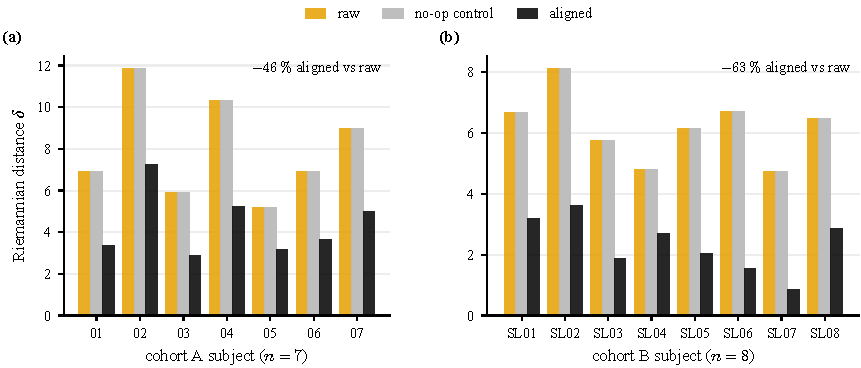
\includegraphics[width=\textwidth]{../results/fig_drift.pdf}
\caption{Session-drift reduction per participant. Bars are the Riemannian
distance $\delta$ between the fitting-session mean covariance and the held-out
session mean, for the raw signal, the momentum-0 no-op control, and the aligned
signal. (a) cohort A, $n=7$; (b) cohort B, $n=8$. Distance falls in every
participant of both cohorts; the no-op control, which shares every code path but
never updates its estimate, shows no reduction.}
\label{fig:drift}
\end{figure*}

\begin{table}[t]
\caption{Session-drift reduction. The no-op control shares every code path but
never updates its estimate. Reduction is mean $\pm$ SD over participants; $p$
from a two-sided paired $t$-test.}
\label{tab:drift}
\centering
\begin{tabular}{lrrrl}
\toprule
Cohort & Raw & Aligned & No-op & Reduction \\
\midrule
A ($n{=}7$) & 8.372 & 4.082 & 9.173 & $52.0\pm4.5\,\%$ \\
B ($n{=}8$) & 6.479 & 1.074 & 6.309 & $83.9\pm3.9\,\%$ \\
\bottomrule
\end{tabular}
\end{table}

\begin{table}[t]
\caption{Per-participant session drift. $\delta$ is the Riemannian distance
(\ref{eq:riem}) between the fitting-session mean covariance and the mean over
held-out sessions. The no-op control shares every code path but never updates
its estimate. Every participant improves.}
\label{tab:persubject}
\centering
\begin{tabular}{lrrrr}
\toprule
Participant & Raw & No-op & Aligned & Reduction \\
\midrule
\multicolumn{5}{l}{\textit{Cohort A, 6 held-out sessions each}}\\
sub-01 & 7.154 & 7.938 & 3.144 & $56.1\,\%$ \\
sub-02 & 12.832 & 16.522 & 7.013 & $45.3\,\%$ \\
sub-03 & 6.092 & 6.228 & 2.827 & $53.6\,\%$ \\
sub-04 & 11.035 & 11.981 & 4.840 & $56.1\,\%$ \\
sub-05 & 5.336 & 4.906 & 2.346 & $56.0\,\%$ \\
sub-06 & 7.016 & 6.644 & 3.399 & $51.5\,\%$ \\
sub-07 & 9.139 & 9.990 & 5.007 & $45.2\,\%$ \\
\midrule
\multicolumn{5}{l}{\textit{Cohort B, 2 held-out trials each}}\\
SL01 & 5.845 & 5.450 & 1.039 & $82.2\,\%$ \\
SL02 & 7.795 & 8.850 & 1.451 & $81.4\,\%$ \\
SL03 & 6.030 & 5.934 & 0.713 & $88.2\,\%$ \\
SL04 & 8.158 & 4.486 & 1.933 & $76.3\,\%$ \\
SL05 & 5.823 & 6.799 & 0.666 & $88.6\,\%$ \\
SL06 & 6.482 & 7.722 & 0.888 & $86.3\,\%$ \\
SL07 & 4.738 & 4.849 & 0.653 & $86.2\,\%$ \\
SL08 & 6.966 & 6.378 & 1.250 & $82.1\,\%$ \\
\bottomrule
\end{tabular}
\end{table}

Drift is reduced in 15 of 15 participants ($t=-9.14$, $p=1\times10^{-4}$ for
cohort A; $t=-20.59$, $p<1\times10^{-5}$ for cohort B), with per-participant
reductions spanning $45.2$ to $56.1\,\%$ on cohort A and $76.3$ to $88.6\,\%$ on
cohort B (Table~\ref{tab:persubject}). No participant regresses, and the
reduction is not carried by one or two outliers. The no-op control shows
no reduction in either cohort, which establishes that the effect comes from
adaptation rather than from the whitening operation or from the measurement
itself. The mechanism works as designed, and Section~\ref{sec:external} shows
that this does not settle whether it helps the task.

\subsection{Component ablation, cohort A}

\begin{figure*}[t]
\centering
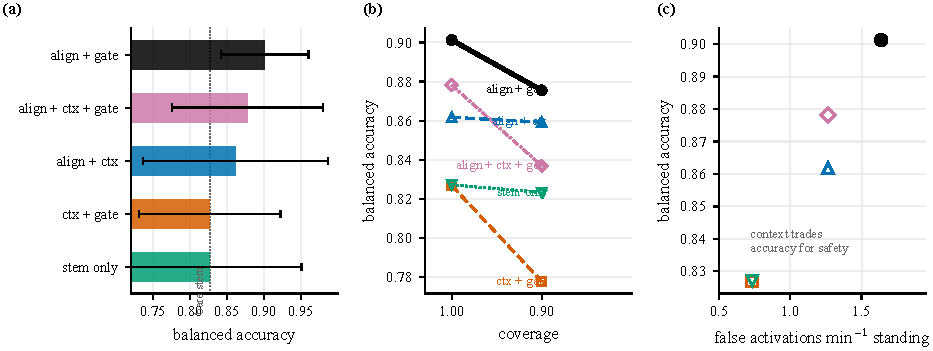
\includegraphics[width=\textwidth]{../results/fig_ablation.pdf}
\caption{Component ablation on cohort A, seed 0. (a) Balanced accuracy by arm;
error bars are $\pm1$ SD across the 7 participants, not across seeds. (b)
Accuracy recovered by declining the least-confident $10\,\%$ of windows. (c)
Balanced accuracy against spurious activations per minute of standing, showing
the cross-epoch context as a selectable operating point.}
\label{fig:ablation}
\end{figure*}

\begin{table}[t]
\caption{Component ablation, cohort A, single seed. Accuracy is the mean over 7
participants with the between-subject SD. Acc@90 is accuracy at $90\,\%$
coverage; FA/min is spurious activations per minute of standing. All cells use
the original estimator so that arms are mutually comparable.}
\label{tab:ablation}
\centering
\begin{tabular}{llrrr}
\toprule
Components & Acc $\pm$ SD & ECE & Acc@90 & FA/min \\
\midrule
align + gate       & $\mathbf{0.901}\pm0.059$ & $\mathbf{0.039}$ & $\mathbf{0.876}$ & 1.64 \\
align + ctx + gate & $0.878\pm0.102$ & 0.074 & 0.837 & 1.26 \\
align + ctx        & $0.862\pm0.125$ & 0.072 & --- & 1.26 \\
ctx + gate         & $0.827\pm0.096$ & 0.091 & 0.778 & 0.73 \\
stem only          & $0.827\pm0.124$ & 0.082 & 0.823 & 0.73 \\
\bottomrule
\end{tabular}
\end{table}

The acc@90 value for the \textit{align + ctx} arm is withheld because with the
selection head disabled the model emits near-constant confidence, so ranking by
it selects the first $90\,\%$ of the test set in recording order. That number
would be an ordering artefact, not a selective accuracy.

\paragraph{Alignment is necessary, not additive} With alignment removed, the
context and selection modules together contribute between $0.000$ and $0.007$:
the no-align arm spans $0.827$--$0.834$ across repeats (Table~\ref{tab:noise})
while the stem-only arm is deterministic at $0.827$. Against the $0.010$ noise
floor that is indistinguishable from nothing, and an order of magnitude below
alignment's own contribution of $+0.028$ to $+0.051$ depending on estimator
version. The modules do not stack; they depend on the alignment stage to be
useful at all.

\paragraph{Cross-epoch context is an operating point} Adding it costs $0.023$
accuracy and raises ECE from $0.039$ to $0.074$, while reducing spurious
activations from $1.64$ to $1.26$ per minute, a $23\,\%$ reduction. We therefore
report it as a selectable safety mode rather than as part of the default
configuration. Removing it also removes 594{,}816 of the model's 618{,}997
parameters, which is what makes the default configuration compact.

\subsection{Comparison with published decoders}
\label{sec:compare}

\begin{figure}[t]
\centering
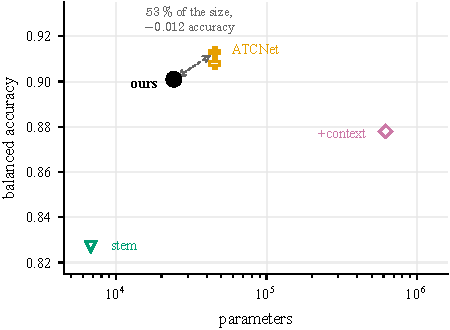
\includegraphics[width=\columnwidth]{../results/fig_efficiency.pdf}
\caption{Balanced accuracy against parameter count on cohort A, single seed,
pipeline C only. The proposed configuration sits $0.012$ below ATCNet at
$53\,\%$ of its parameters. No point from the other pipeline appears here.}
\label{fig:efficiency}
\end{figure}

\begin{table}[t]
\caption{Cohort A comparison. Groups are separated by training pipeline and must
not be compared across the rule; ATCNet appears in both and differs by $0.032$.
Pipeline C is single seed; pipeline F is the mean of 2 seeds with the per-seed
range in brackets.}
\label{tab:compare}
\centering
\begin{tabular}{lrl}
\toprule
Model & Params & Bal. acc. \\
\midrule
\multicolumn{3}{l}{\textit{Pipeline C (this work), seed 0}}\\
ATCNet \citep{atcnet}                & 45{,}280 & \textbf{0.913} \\
ATCNet, rate-matched kernels         & 45{,}280 & 0.908 \\
\textbf{Ours, align + gate}          & \textbf{24{,}181} & 0.901 \\
Ours, align + ctx + gate             & 618{,}997 & 0.878 \\
Ours, stem only                      & 6{,}768  & 0.827 \\
\midrule
\multicolumn{3}{l}{\textit{Pipeline F (earlier), mean of 2 seeds}}\\
ATCNet \citep{atcnet}                & 45{,}280 & 0.879 [0.876--0.881] \\
EEGNeX \citep{eegnex}                & 58{,}082 & 0.876 [0.855--0.896] \\
ShallowFBCSPNet \citep{schirrmeister}& 97{,}120 & 0.867 [0.856--0.877] \\
EEG Conformer \citep{conformer}      & 440{,}706 & 0.843 [0.834--0.852] \\
\bottomrule
\end{tabular}
\end{table}

In the pipeline where both were measured, ATCNet scores $0.913$ against $0.901$
at seed 0 and $0.892$ for our two-seed mean (Table~\ref{tab:seeds}). The gap of
$0.012$ to $0.021$ sits inside the $0.020$ between-seed spread of
Section~\ref{sec:noise}, so two seeds cannot separate the two models. We report
it as a loss rather than as a tie because the point estimate favours ATCNet in
both seeds we ran.

\paragraph{The modules do not transfer to another backbone} If the selection and
context modules were generally useful, attaching them to a stronger backbone
should help. They do not: stock ATCNet with our cross-epoch context and
selective head scores $0.894$ against $0.913$ for stock ATCNet alone, a loss of
$0.018$ (Table~\ref{tab:atcours}). The modules improve calibration
($\mathrm{ECE}$ $0.058$, and an abstention point at $0.849$) and cost accuracy,
which is the same trade seen within our own architecture in
Table~\ref{tab:ablation}, and it is a trade, not an improvement.

\begin{table}[t]
\caption{Attaching our two modules to a stronger backbone, cohort A, single
seed. Stock ATCNet has no selection head, so no abstention operating point is
defined for it.}
\label{tab:atcours}
\centering
\begin{tabular}{lrrr}
\toprule
Model & Acc & ECE & Acc@90 \\
\midrule
Stock ATCNet \citep{atcnet}    & \textbf{0.913} & --- & --- \\
ATCNet + ctx + selective head  & 0.894 & 0.058 & 0.849 \\
ATCNet, rate-matched kernels   & 0.908 & --- & --- \\
\bottomrule
\end{tabular}
\end{table}

What the configuration offers
instead is parity with the strongest baseline at $53\,\%$ of its parameters and
$5\,\%$ of EEG Conformer's (Fig.~\ref{fig:efficiency}), together with calibrated
confidence ($\mathrm{ECE}=0.039$) and a trained abstention operating point
($0.876$ at $90\,\%$ coverage), neither of which the baselines provide. We note
that the baselines were not compressed for this comparison, so the parameter
axis reports what the published architectures cost, not their achievable
minimum.

\subsection{External validation: the ordering inverts}
\label{sec:external}

\begin{figure}[t]
\centering
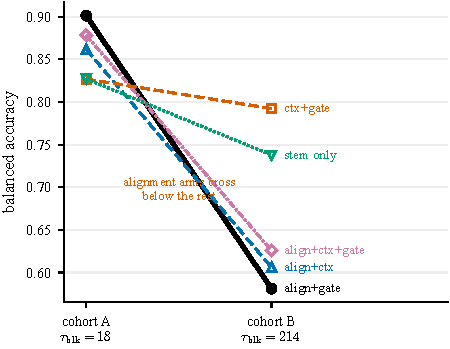
\includegraphics[width=\columnwidth]{../results/fig_inversion.pdf}
\caption{The same five arms on both cohorts, single seed. Solid heavy black is
the proposed configuration; the other alignment-using arms are dashed in colour,
and the two alignment-free arms are dashed and dotted. The three alignment arms
cross below both alignment-free arms, so the ordering inverts rather than
compressing.}
\label{fig:inversion}
\end{figure}

\begin{table}[t]
\caption{Both cohorts, single seed, original estimator.}
\label{tab:external}
\centering
\begin{tabular}{lrr}
\toprule
Components & Cohort A & Cohort B \\
\midrule
align + gate       & \textbf{0.901} & 0.581 \\
align + ctx + gate & 0.878 & 0.626 \\
align + ctx        & 0.862 & 0.606 \\
ctx + gate         & 0.827 & \textbf{0.792} \\
stem only          & 0.827 & 0.737 \\
\bottomrule
\end{tabular}
\end{table}

On cohort B the bare stem outperforms the full model, $0.737$ against $0.626$,
and the best cohort-A configuration is the worst cohort-B one. The ordering does
not merely compress; it inverts, and the three arms that use alignment fall
below both arms that do not. We report this in full rather than restricting the
paper to the cohort on which the architecture succeeds, and the remainder of the
results explains it, because the explanation turns out to be the more
transferable contribution.

\subsection{Interventions tested and rejected}
\label{sec:rejectedset}

Six architectural interventions were tested before the configuration reported
here and rejected by their own controls (Table~\ref{tab:rejected}). We report
them because each control is what distinguishes a mechanism from a correlation,
and because two of them looked convincing until the control was run.

\begin{table}[t]
\caption{Interventions tested and rejected, each by a pre-specified control.
Cohort A unless stated. The motion-cancellation row is the clearest case: the
module scored $0.905$ with the inertial channel present and chance with it
zeroed, so it was an inertial classifier, not an EEG one.}
\label{tab:rejected}
\centering
\small
\begin{tabular}{lll}
\toprule
Intervention & Control & Outcome \\
\midrule
Motion cancellation & inertial input zeroed & $0.905 \rightarrow 0.501$ \\
                    & inertial input shuffled & $0.905 \rightarrow 0.529$ \\
Amplitude side-channel & label-shuffled control & control matches \\
ShallowFBCSP $\times$ ATCNet & vs EEG Conformer & $0.848$ vs $0.843$ \\
Capacity scaling & 19k--441k parameters & no trend \\
MRCP dual-band pathway & vs ERD alone & $0.742$ vs $0.775$ \\
Within-epoch attention & ablate the attention & $+0.024$ to remove \\
\bottomrule
\end{tabular}
\end{table}

The movement-related cortical potential (MRCP) pathway deserves a sentence
because it is a physiologically motivated design that failed cleanly. Decoding
from the 0.1--3\,Hz onset-locked band alone gives $0.604$; from the mu and beta
ERD band alone, $0.775$; combining the two, $0.742$. The paired difference
between the combination and the better single band is $-0.034$, so on
single-trial data the low-frequency pathway adds noise rather than information,
and the architecture uses the ERD band only.

\subsection{A rejected explanation for the inversion}
\label{sec:rejected}

Our first diagnosis was the power-weighted estimator described in
Section~\ref{sec:align}. The defect is real and measurable: on cohort B, where
the majority class carries $1.52\times$ the power, the un-normalised running
estimate sat at Riemannian distance $0.306$ from the walk covariance, which is
to say it had become the majority class. The per-window trace normalisation in
(\ref{eq:update}) moves it to $3.899$ and $3.194$ from the two class
covariances.

Correcting it changed decoding by $+0.005$ on cohort B and $-0.016$ on cohort A.
The estimator improved and the task did not follow, so we reject this as the
explanation for the inversion while retaining the correction, which is
independently right. We report it because it is the first of five cases in this
work where a distribution-level quantity improved without the task following
(Section~\ref{sec:discussion}).

\subsection{The adaptation rate condition}
\label{sec:rate}

\paragraph{Diagnosis} The running estimate tracks whatever is currently
streaming. An exponential moving average with momentum $m$ has an effective
memory of approximately $1/m$ batches, or $NB/m$ windows at batch size $N$ and
$B$ batches. When a protocol presents a class in contiguous blocks longer than
that memory, the estimate converges to the currently streaming class, and
whitening by it removes the between-class difference. Cohort A's blocks
($\tau_{\mathrm{blk}}=18$) sit far inside even the fastest memory; cohort B's
($\tau_{\mathrm{blk}}=309$) do not.

\paragraph{Prediction} Slowing adaptation until the memory exceeds a class block
should restore cohort B. The memory is approximately 160, 640 and 3200 windows
at $m=0.2$, $0.05$ and $0.01$, so the crossing of
$\tau_{\mathrm{blk}}=309$ falls between the first and second settings.

\begin{table}[t]
\caption{Momentum sweep, cohort B, all five arms, single seed. ``At crossing''
is $m{=}0.20 \rightarrow 0.05$, where the estimator memory passes the 309-window
class block. Every arm that uses alignment gains; neither arm that omits it
responds.}
\label{tab:sweep}
\centering
\begin{tabular}{lrrrrc}
\toprule
Arm & $0.20$ & $0.05$ & $0.01$ & At crossing & Aligns \\
\midrule
align+ctx+gate & 0.626 & 0.724 & 0.723 & $\mathbf{+0.098}$ & yes \\
align+gate     & 0.581 & 0.671 & 0.696 & $\mathbf{+0.090}$ & yes \\
align+ctx      & 0.606 & 0.700 & 0.726 & $\mathbf{+0.094}$ & yes \\
ctx+gate       & 0.792 & 0.782 & 0.783 & $-0.010$ & no \\
stem only      & 0.737 & 0.737 & 0.737 & $\mathbf{0.000}$ & no \\
\bottomrule
\end{tabular}
\end{table}

\begin{figure*}[t]
\centering
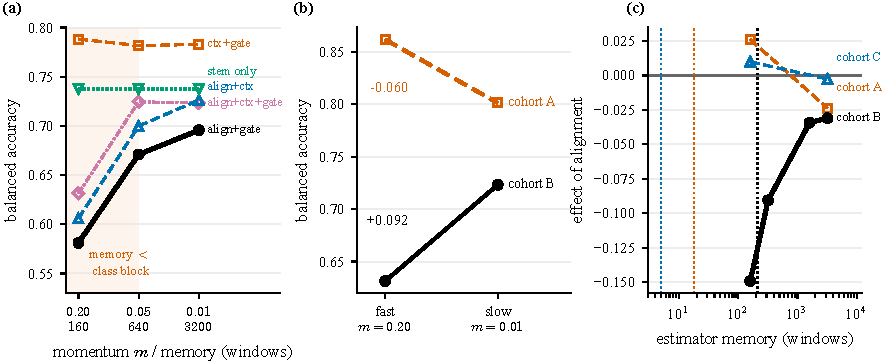
\includegraphics[width=\textwidth]{../results/fig_rate.pdf}
\caption{The adaptation rate condition. (a) Cohort B, five arms, three momenta,
single seed; the shaded region is where the estimator memory is shorter than a
class block. Measurement points are marked because the sweep is sparse. (b) The
same change applied to both cohorts at matched estimator version, giving
opposite signs. (c) The admissible band of Proposition~\ref{prop:band}, bounded
below by $\tau_{\mathrm{blk}}$ and above by $\tau_{\mathrm{drift}}$; the upper
bound is bracketed by cohort A being good at 160 windows and poor at 3200, not
pinned.}
\label{fig:rate}
\end{figure*}

Every arm that uses alignment gains $+0.090$ to $+0.098$ as the memory crosses
the class-block length (Table~\ref{tab:sweep}). Neither arm that omits alignment
responds: the no-align arm moves $-0.010$, within its $0.0107$ run-to-run spread
(Table~\ref{tab:noise}), and the stem-only arm reproduces $0.7375$ exactly at
every setting despite a 160-fold change in the adaptation rate. Because that arm
is deterministic, this is an exact null rather than an unresolved one. The
manipulated variable therefore acts only through the component it controls,
which an unrelated confound such as optimisation dynamics or regularisation
would not produce.

\subsection{The condition is two-sided}
\label{sec:twosided}

We predicted, and recorded the prediction before running it, that the same
change would be free on cohort A, whose blocks sit far inside even the fastest
memory so that the estimate was already class-mixed. It is not
(Table~\ref{tab:twosided}).

\begin{table}[t]
\caption{The same momentum change applied to both cohorts at matched estimator
version, single seed. Deltas are computed at full precision, not from the
rounded cells.}
\label{tab:twosided}
\centering
\begin{tabular}{lrrr}
\toprule
Cohort & $m=0.20$ & $m=0.01$ & $\Delta$ \\
\midrule
A ($\tau_{\mathrm{blk}}=18$)  & \textbf{0.862} & 0.801 & $\mathbf{-0.060}$ \\
B ($\tau_{\mathrm{blk}}=309$) & 0.631 & \textbf{0.723} & $\mathbf{+0.092}$ \\
\bottomrule
\end{tabular}
\end{table}

The optima are opposite, and error in either direction costs $0.060$ to $0.092$,
six to nine times the noise floor. The prediction failed because it accounted
only for the harm a fast estimate can do and not for the benefit it was
delivering, which is tracking genuine session drift.

\begin{proposition}[Admissible rate band]
\label{prop:band}
A running covariance estimate with effective memory $\mu$ windows both avoids
tracking the streaming class and tracks session drift only if
\begin{equation}
\tau_{\mathrm{blk}} \;<\; \mu \;<\; \tau_{\mathrm{drift}} .
\label{eq:band}
\end{equation}
Where $\tau_{\mathrm{blk}} \ge \tau_{\mathrm{drift}}$ the band is empty and no
setting of $\mu$ satisfies both requirements.
\end{proposition}

Cohort A satisfies (\ref{eq:band}) with a wide margin, so fast adaptation is
both safe and useful there, and slowing it forfeits the drift tracking for no
compensating gain. Cohort B's 309-window blocks force $\mu$ slow enough that it
can no longer track drift, so the band is empty.

\begin{remark}[The residual]
This accounts for the residual without a third mechanism. Even at its best
setting, alignment still costs $0.060$ on cohort B ($0.723$ against $0.783$ for
the no-align arm), because at the only rate that avoids class tracking there is
no drift-tracking benefit left to collect. The layer then contributes only
estimation noise.
\end{remark}

\begin{remark}[Why offline alignment does not meet this failure]
A whole-recording estimate, as in Euclidean Alignment \citep{hewu}, is the
maximally slow setting. It therefore never tracks the class, and it never tracks
within-recording drift either, which is exactly the capability an in-network
version is introduced to add. The failure mode is created by the move that
creates the benefit.
\end{remark}

Both bounds in (\ref{eq:band}) are properties of the recording protocol.
$\tau_{\mathrm{blk}}$ is read off the trial structure, and $\tau_{\mathrm{drift}}$
is estimated from the Riemannian distance between session covariances, which
needs no labels. The condition is therefore checkable before a model is fitted.

%=============================================================================
\section{Discussion}
\label{sec:discussion}

\subsection{Mechanism validation is not performance validation}

Domain adaptation and invariance methods are routinely justified by a
distribution-level quantity, a divergence, an alignment distance or a
nuisance-decodability score, with task performance assumed to follow
\citep{ganin,long,coral,bendavid}. This work provides five counterexamples
within a single system, three of which we produced by acting on that assumption
ourselves (Fig.~\ref{fig:metrics}).

\begin{figure}[t]
\centering
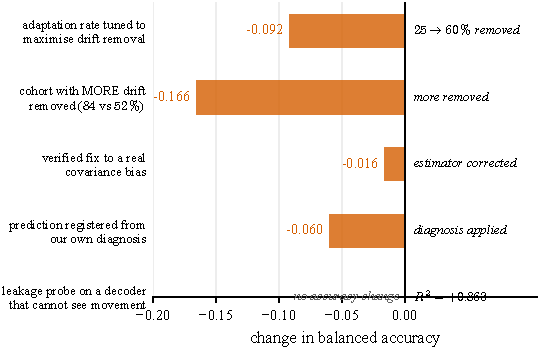
\includegraphics[width=\columnwidth]{../results/fig_metrics.pdf}
\caption{Five cases in which a distribution-level quantity improved (right, in
blue) and the task did not follow (left, in red). The final row has no accuracy
change and therefore no bar: the leakage probe rises with accuracy whether or
not the decoder can access the nuisance.}
\label{fig:metrics}
\end{figure}

\begin{enumerate}
\item The adaptation rate was originally selected because it maximised drift
      reduction ($60\,\%$ against $25\,\%$). That choice cost $0.092$ accuracy
      on cohort B (Table~\ref{tab:sweep}).
\item The cohort in which more drift was removed ($83.9\,\%$ against
      $52.0\,\%$, Table~\ref{tab:drift}) is the cohort in which accuracy fell by
      $0.166$ (Table~\ref{tab:external}).
\item A verified correction to a genuine covariance-estimation bias moved
      decoding by $+0.005$ and $-0.016$ (Section~\ref{sec:rejected}).
\item A prediction registered from our own diagnosis was falsified
      (Table~\ref{tab:twosided}), because the diagnosis accounted only for the
      harm the estimate can do.
\item The nuisance-leakage probe rises with accuracy whether or not the decoder
      can access the nuisance, measuring $R^2=+0.863$ for one that cannot.
\end{enumerate}

Item 4 generalises the rest. Each of these quantities is one-sided by
construction: it scores the failure it was designed to detect and carries no
term for the capability the intervention removes. Drift reduction measures how
much non-stationarity a layer removes and has no term for what the layer
destroys. A diagnosis inherited from such a metric inherits its blind spot,
which is why our own threshold rule was correct about one direction and silent
about the other until we tested it where it predicted no effect. The practical
implication is that reporting a reduced divergence, increased invariance or
lowered nuisance decodability is evidence about the representation and not
evidence that the method helps, even when the reduction is large and
reproducible.

\subsection{Relation to temporally correlated test-time adaptation}

The vision literature has identified that test-time adaptation degrades when the
test stream is temporally correlated \citep{note,sar,cotta}, and proposes
reservoirs and stabilised objectives as remedies. Our result is compatible with
that line and adds two things specific to the blocked-protocol case. First, the
relevant quantity is a ratio of timescales rather than a qualitative property of
the stream, and the threshold location is predicted rather than fitted
(Table~\ref{tab:sweep}). Second, the constraint is two-sided, because in a
longitudinal deployment the same estimator that can track the class is also the
one that tracks the drift, so the remedies that slow adaptation trade one
failure for the other rather than removing both.

%=============================================================================
\section{Limitations}
\label{sec:limits}

We state the objections a reviewer should raise, because each is a real
constraint on what the results support.

\textbf{Single seed.} The ablations are seed 0. With a $0.010$ noise floor on
transformer-containing arms (Table~\ref{tab:noise}), single-seed rankings of
closely spaced models are not interpretable, and we avoid making them: the
$0.012$ gap to ATCNet in Table~\ref{tab:compare} is reported as a loss rather
than resolved in either direction. The effects we do interpret ($+0.090$ to
$+0.098$, $-0.060$) are six to ten times that floor. Multi-seed replication of
the headline ablation remains outstanding.

\textbf{No paired significance tests on accuracy.} Per-participant accuracies
were not retained, only the mean and between-subject SD, so the accuracy
comparisons carry dispersion but not paired tests. The drift results
(Table~\ref{tab:drift}) are paired and tested; the accuracy comparisons are not.

\textbf{Cohort size.} Seven and eight participants. This is typical for
exoskeleton BCI studies \citep{he_exo} but small, and the between-subject SD of
$0.06$ to $0.13$ (Table~\ref{tab:ablation}) is large relative to the differences
between arms.

\textbf{Best-epoch evaluation.} Model selection uses the best epoch by held-out
balanced accuracy, which is conventional but upward-biased on small folds. The
bias applies equally to all arms and baselines within a pipeline, so comparisons
within a pipeline are unaffected, but absolute values should be read as
optimistic.

\textbf{The upper bound is bracketed, not measured.}
$\tau_{\mathrm{drift}}$ in (\ref{eq:band}) is bounded by cohort A performing
well at a 160-window memory and poorly at 3200. We have not measured an interior
optimum, and a cohort whose admissible band is narrow but non-empty would test
Proposition~\ref{prop:band} properly.

\textbf{The rule is post-hoc.} Proposition~\ref{prop:band} was derived after
observing cohort B fail. One prediction from it has since been tested
out-of-sample, and that test falsified the one-sided form
(Table~\ref{tab:twosided}), which is how the two-sided form arose. The corrected
form has not yet predicted anything in advance.

\textbf{Window length differs between cohorts.} Cohort B uses 2\,s windows
against cohort A's 4\,s, so the context pathway spans a shorter duration there.
This is a confound for the context ablation specifically, though not for the
rate condition, which is measured within each cohort.

%=============================================================================
\section{Conclusion}

An estimate that adapts at test time tracks whatever is currently streaming.
Under a blocked experimental protocol that includes the class label, and the
layer then removes the signal it was inserted to protect. The rate at which it
adapts must exceed the class-block timescale and remain below the drift
timescale, and where those requirements cross no admissible rate exists. Both
bounds are read from the recording protocol, which makes this a design-time
check.

The immediate open question is whether the band in (\ref{eq:band}) has an
interior optimum that can be located rather than bracketed. Neither cohort here
can answer it: cohort A's band is wide enough that the fastest setting tested is
already inside it, and cohort B's is empty. A protocol with
$\tau_{\mathrm{blk}}$ between roughly 100 and 200 windows would place the two
bounds close together, and the prediction is that accuracy would peak at an
intermediate momentum and fall on both sides. That experiment is pre-registrable
from the protocol alone, and it is the test we would want before treating
Proposition~\ref{prop:band} as established rather than as a description of two
cohorts.

A second direction follows from the residual. If a single running estimate
cannot simultaneously avoid the class and track the drift, then the two
requirements should perhaps be served by two estimators at different rates, with
the fast one constrained to the subspace in which drift lives and the slow one
supplying the class-neutral reference. Whether such a decomposition is
identifiable without labels is open, and it is the version of this architecture
we would build next.

Finally, the broader caution transfers beyond EEG. Five times in this system a
distribution-level quantity improved while the task did not follow, and in three
of those cases we had acted on the assumption that it would. Such metrics are
one-sided by construction. Any method justified by a reduced divergence should
report what the reduction costs, and any diagnosis inherited from one should be
tested in the direction where it predicts nothing will happen.

%=============================================================================
\section*{CRediT authorship contribution statement}
\textbf{Author Name}: Conceptualization, Methodology, Software, Validation,
Formal analysis, Investigation, Data curation, Writing -- original draft,
Writing -- review and editing, Visualization.

\section*{Declaration of competing interest}
The authors declare no known competing financial interests or personal
relationships that could have appeared to influence the work reported in this
paper.

\section*{Data availability}
Both datasets are publicly available. All code, configurations and result files,
including those of experiments that failed, are in the accompanying repository.

\bibliographystyle{cas-model2-names}
\bibliography{refs}

\end{document}
